\documentclass[aspectratio=169]{beamer}

\usepackage{ctex}
\usepackage{amsmath,amsfonts,amssymb,bm}
\usepackage{graphicx}
\usepackage{booktabs}
\usepackage{tabularx}
\usepackage{array}
\usepackage{ragged2e}
\usepackage{hyperref}
\usepackage{pgfpages}
\usepackage{xcolor}

\usetheme{Berlin}
\usecolortheme{whale}
\useinnertheme[shadow=true]{rounded}
\usefonttheme[onlymath]{serif}
\setbeamercovered{transparent}
\setbeamertemplate{navigation symbols}{}
\hypersetup{hidelinks}

\newcolumntype{Y}{>{\RaggedRight\arraybackslash}X}
\newcommand{\best}[1]{\textbf{\color{blue!65!black}#1}}
\newcommand{\risk}[1]{\textbf{\color{red!70!black}#1}}
\newcommand{\postperiod}[1]{\textbf{\color{orange!85!black}#1}}
\newcommand{\evidence}[1]{\par\vspace{1mm}{\tiny\color{black!58}证据：#1}}
\newcommand{\done}{\textbf{\color{green!55!black}已完成}}
\newcommand{\partdone}{\textbf{\color{orange!85!black}部分完成}}
\newcommand{\notdone}{\textbf{\color{red!70!black}未完成}}
\graphicspath{{figures/semiannual_report_2026h1/}}

\makeatletter
\newif\ifpympressnotesright
\newif\ifpympressnotesafter
\newif\ifreportappendix
\reportappendixfalse
\@ifundefined{pympressnotesright}{\pympressnotesrightfalse}{\pympressnotesrighttrue}
\@ifundefined{pympressnotesafter}{\pympressnotesafterfalse}{\pympressnotesaftertrue}
\makeatother
\ifpympressnotesright
  \setbeameroption{show notes on second screen=right}
\else\ifpympressnotesafter
  \setbeameroption{show notes}
\else
  \setbeameroption{hide notes}
\fi\fi
\newcommand{\speakernote}[1]{\note{\footnotesize\sloppy #1}}
\newcommand{\pageindicator}{%
  \ifreportappendix
    附件~\number\numexpr\insertframenumber-14\relax/3%
  \else
    \insertframenumber/14%
  \fi}

\setbeamertemplate{footline}{%
 \leavevmode%
 \hbox{%
 \begin{beamercolorbox}[wd=.31\paperwidth,ht=2.25ex,dp=1ex,center]{author in head/foot}
 \insertshortauthor
 \end{beamercolorbox}%
 \begin{beamercolorbox}[wd=.38\paperwidth,ht=2.25ex,dp=1ex,center]{title in head/foot}
 \insertshorttitle
 \end{beamercolorbox}%
 \begin{beamercolorbox}[wd=.31\paperwidth,ht=2.25ex,dp=1ex,center]{date in head/foot}
 \insertshortdate \quad \pageindicator
 \end{beamercolorbox}%
 }
}

\title[2026 年上半年综合汇报]{2026 年上半年研究与发展综合汇报}
\subtitle{晶体带隙 GNN：从模型探索、数据审计到论文初稿}
\author[刘嘉瑞｜内部材料]{汇报人：刘嘉瑞}
\institute[物理人工智能]{物理系研究生｜2026 年秋季进入研二\\研究方向：物理人工智能｜评价周期：2026 年 1 月—6 月\\发展路径：学术主线 + 工程准入（复合型倾向）}
\date{2026 年 8 月}

\begin{document}

% 正文 1
\begin{frame}
  \titlepage
  \vspace{-3mm}
  \begin{center}
    {\small\color{red!75!black}\textbf{内部汇报材料，请勿对外传播}}
  \end{center}
  \speakernote{各位老师好，我是刘嘉瑞，物理系研究生，今年秋季进入研二。本次汇报复盘的是 2026 年 1 月到 6 月。我的主线是晶体带隙预测图神经网络研究，目标是把模型实验、跨数据源审计和论文写作连成一个可验证的研究闭环。发展路径上，我希望继续以学术研究为主，同时申请进入工程项目，因此这里按复合型倾向汇报，但学术成果与工程能力分开计算。}
\end{frame}

\section{个人与目标}

% 正文 2
\begin{frame}[shrink=8]{本评价周期目标与完成情况}
\small
\begin{alertblock}{口径说明}
周期初\textbf{没有正式书面 KPI}。以下目标根据 6 月 30 日前的可核验产物回溯整理，核心意图是：\best{形成一项可投稿的机器学习研究工作}。
\end{alertblock}

\begin{tabularx}{\textwidth}{p{5.0cm} p{2.3cm} Y}
\toprule
回溯目标 & 状态 & 截至 2026-06-30 的证据 \\
\midrule
建立可复现实验框架与强基线 & \done & CGCNN、ALIGNN、M3GNet；统一配置、指标和预测输出。 \\
验证全局信息与物理增强是否有效 & \done & E/S/T 系列消融；结论从“堆复杂模型”收敛到 simple VN + Huber。 \\
解决 MP/HZW 迁移矛盾并形成数据结论 & \done & structure-first audit、双标签同结构验证。 \\
形成论文初稿并完成投稿 & \partdone & 6 月形成 15 页中文初稿；\risk{周期内尚未投稿}。 \\
进入正式工程项目 & \notdone & 上半年无正式任务书或验收；下一周期申请进入。 \\
\bottomrule
\end{tabularx}
\speakernote{周期初没有书面 KPI，所以我不把后来完成的事情伪装成原定考核项，而是根据文件和结果回溯目标。前三项已经形成闭环：框架、实验结论和数据审计都有可核验产物。论文方面，六月已经形成十五页中文初稿，但没有在上半年完成投稿，因此只能算部分完成。工程项目方面，上半年没有正式任务书和验收记录，不能把研究代码直接算成工程项目绩效；我的意向是在下一周期正式申请进入。}
\end{frame}

% 正文 3
\begin{frame}{上半年关键时间线：从方向准备到论文初稿}
\footnotesize
\begin{tabularx}{\textwidth}{p{1.8cm} p{3.4cm} Y}
\toprule
阶段 & 核心动作 & 可验证产物与研究转折 \\
\midrule
1—2 月 & 方向准备期 & 未找到稳定归档产物；本次如实不计完成项。 \\
3 月 & 文献与问题定义 & 梳理 CGCNN、ALIGNN、M3GNet、虚拟节点与长程信息相关工作。 \\
4 月 & 框架重建与模型探索 & 建立 faithful training 框架；完成基线、virtual node、attention、physics 与 size-aware 系列。 \\
5 月 & MP 迁移与数据质量转折 & HZW 上的复杂模型收益未能稳定迁移；转向 MP/HZW structure-first audit，并处理 GPU QOS 阻塞。 \\
6 月 & 双标签验证与论文初稿 & relaxed clean equal-atoms T 系列完成；确认 Huber 跨源稳定；形成 15 页中文论文初稿。 \\
\bottomrule
\end{tabularx}

\begin{block}{这半年真正形成的能力}
从“实现一个模型”推进到：\best{提出假设 → 构造消融 → 发现反例 → 审计数据 → 收敛结论 → 写成论文}。
\end{block}
\speakernote{时间线上，真正有归档证据的工作主要集中在三月到六月。一二月我不虚构项目成果，只记为方向准备期。三月完成文献和问题定义；四月重建训练框架并铺开模型谱系；五月出现关键反例，HZW 的复杂模型收益没有迁移到 MP，于是研究重心从继续堆模型转向审计数据；六月完成同结构双标签验证并形成论文初稿。对我来说，这半年最重要的成长不是多跑了多少模型，而是完成了一次从假设、反例到结论收敛的研究闭环。}
\end{frame}

\section{学术进展}

% 正文 4
\begin{frame}[shrink=2]{研究问题与技术路线}
\small
\begin{columns}[T,onlytextwidth]
\begin{column}{0.48\textwidth}
\begin{block}{研究问题 1：模型}
晶体 band gap 主要依赖局部化学与几何，但 ALIGNN 的局部消息传递是否仍缺少全局上下文？
\end{block}
\begin{block}{研究问题 2：数据}
相同或对应的 MP/HZW 晶体结构，band gap 标签是否真的等价？标签差异会不会改变模型排序？
\end{block}
\end{column}
\begin{column}{0.50\textwidth}
\begin{alertblock}{技术路线}
\begin{enumerate}
  \item 复现 CGCNN / ALIGNN / M3GNet；
  \item 在 ALIGNN 上加入 single/dual virtual node、attention、physics、routing；
  \item 从 HZW 迁移到 MP，检查结论是否稳定；
  \item 做 structure-first audit，构建同结构双标签数据；
  \item 用 Huber、top-$k$、warmup、decay 做最终消融。
\end{enumerate}
\end{alertblock}
\end{column}
\end{columns}

\begin{center}
\large 模型改进与数据一致性必须\best{同时验证}，否则单一排行榜无法解释。
\end{center}
\speakernote{研究有两条互相约束的主线。模型问题是 ALIGNN 已经能描述局部键角，额外全局信息到底还能不能带来稳定收益；数据问题是 MP 和 HZW 的结构虽然能够对应，但监督标签是否等价。如果只看一个数据集上的最低 MAE，很容易把标签源差异误认为模型创新。因此技术路线不是单纯增加网络复杂度，而是先建立基线，再做模型消融，发现迁移失败后审计数据，最后在同一批结构、两个标签源上重新验证。}
\end{frame}

% 正文 5
\begin{frame}{学术进展一：模型谱系从发散探索收敛到稳定主张}
\scriptsize
\begin{tabularx}{\textwidth}{p{2.3cm} p{4.3cm} Y}
\toprule
阶段 & 代表方案 & 得到的证据 \\
\midrule
强基线 & CGCNN、ALIGNN、M3GNet & ALIGNN 是当前任务最稳定的传统基线。 \\
简单全局通道 & ALIGNN + single plain virtual node & 在 HZW、MP full 和最终双标签口径均有稳定信号。 \\
复杂全局机制 & Transformer、attentive VN、dual slot、size gate、routing & 部分数据或大结构有局部收益，但整体与跨源不稳定。 \\
物理与任务分支 & CBM/VBM constraint、physics branch、metal-aware 等 & 提供探索线索，但标签缺失、任务耦合和复杂度限制了主线价值。 \\
最终消融 & Huber、top-$k$、warmup、global broadcast decay & Huber 是跨 MP/HZW 最稳定增益；decay 只在 MP 上进一步最优。 \\
\bottomrule
\end{tabularx}

\begin{alertblock}{研究结论的变化}
初始假设：“更复杂的全局机制应该更强。”\\
最终主张：\best{简单全局节点 + 鲁棒损失}比复杂注意力或双槽位更稳定。
\end{alertblock}
\speakernote{模型探索并不是每个方案都成功。ALIGNN 是最强传统基线，简单的单 virtual node 是第一条稳定增强。之后我尝试了 Transformer、注意力超节点、双槽位、尺寸监督和路由等复杂机制，它们在某些数据或大结构上有局部信号，但整体不稳定。最终消融显示，真正跨 MP 和 HZW 都能复现的收益来自 Huber 鲁棒损失，而 global decay 只在 MP 标签上更好。这个结果纠正了我最初“复杂机制应该更强”的预设。}
\end{frame}

% 正文 6
\begin{frame}{学术进展二：数据审计解释了模型排序为何改变}
\centering
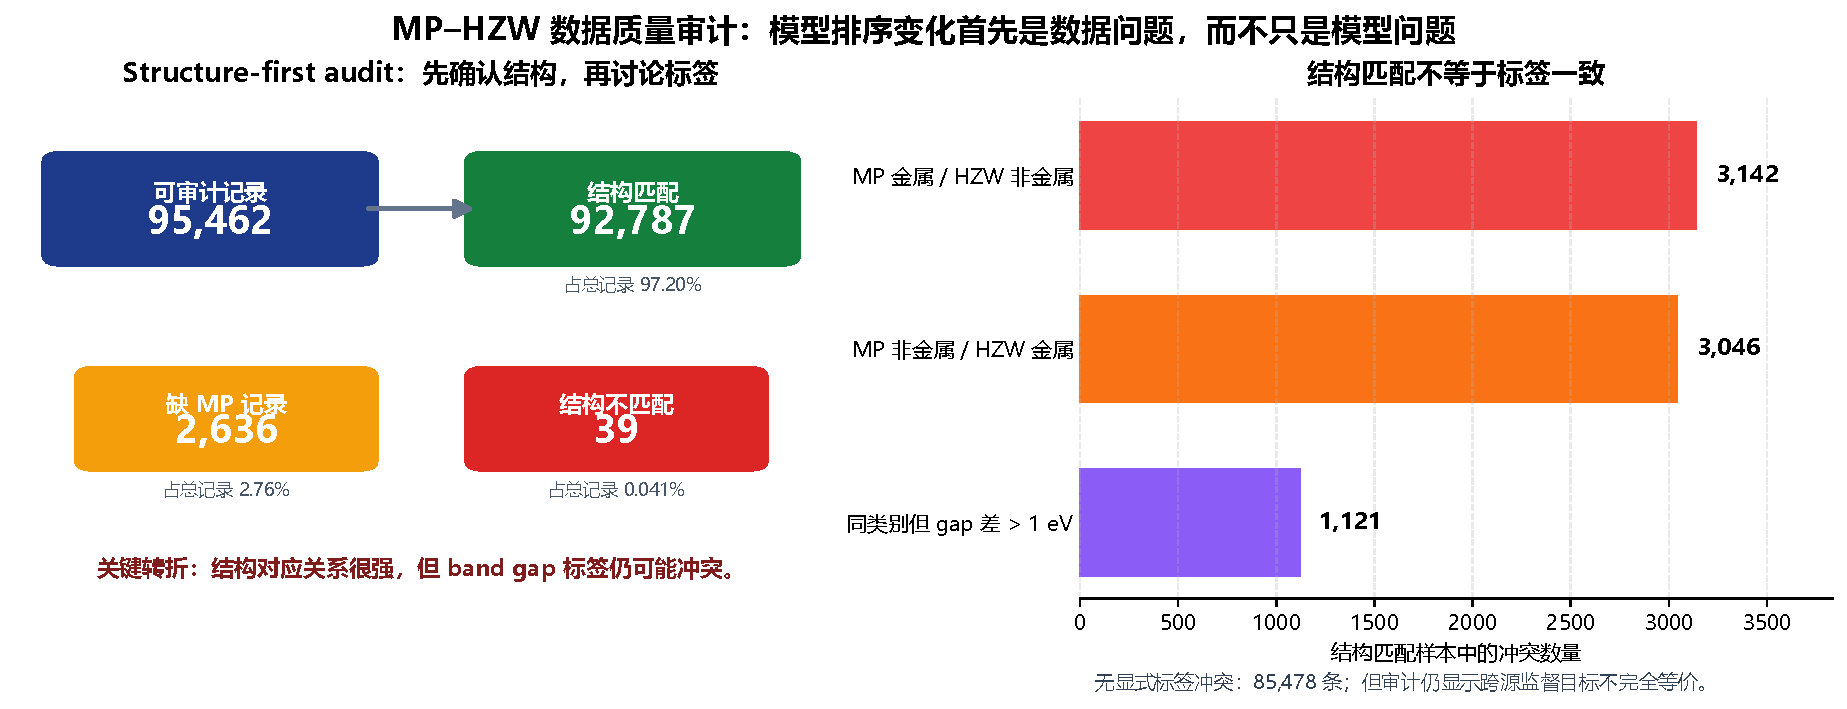
\includegraphics[width=0.96\textwidth]{data_audit_summary.pdf}
\speakernote{这是项目的关键转折。九万五千四百六十二条可审计记录中，九万二千七百八十七条结构能够匹配，结构不匹配只有三十九条，说明结构对应关系很强。但在结构匹配内部，两个标签源仍有三千一百四十二条和三千零四十六条金属非金属冲突，还有一千一百二十一条同类别但带隙差超过一电子伏。也就是说，结构匹配不等于标签一致。模型排序从 HZW 迁移到 MP 后发生变化，首先是数据监督目标改变，而不能简单解释为模型失效。}
\end{frame}

% 正文 7
\begin{frame}{学术进展三：同结构双标签验证给出最终模型结论}
\centering
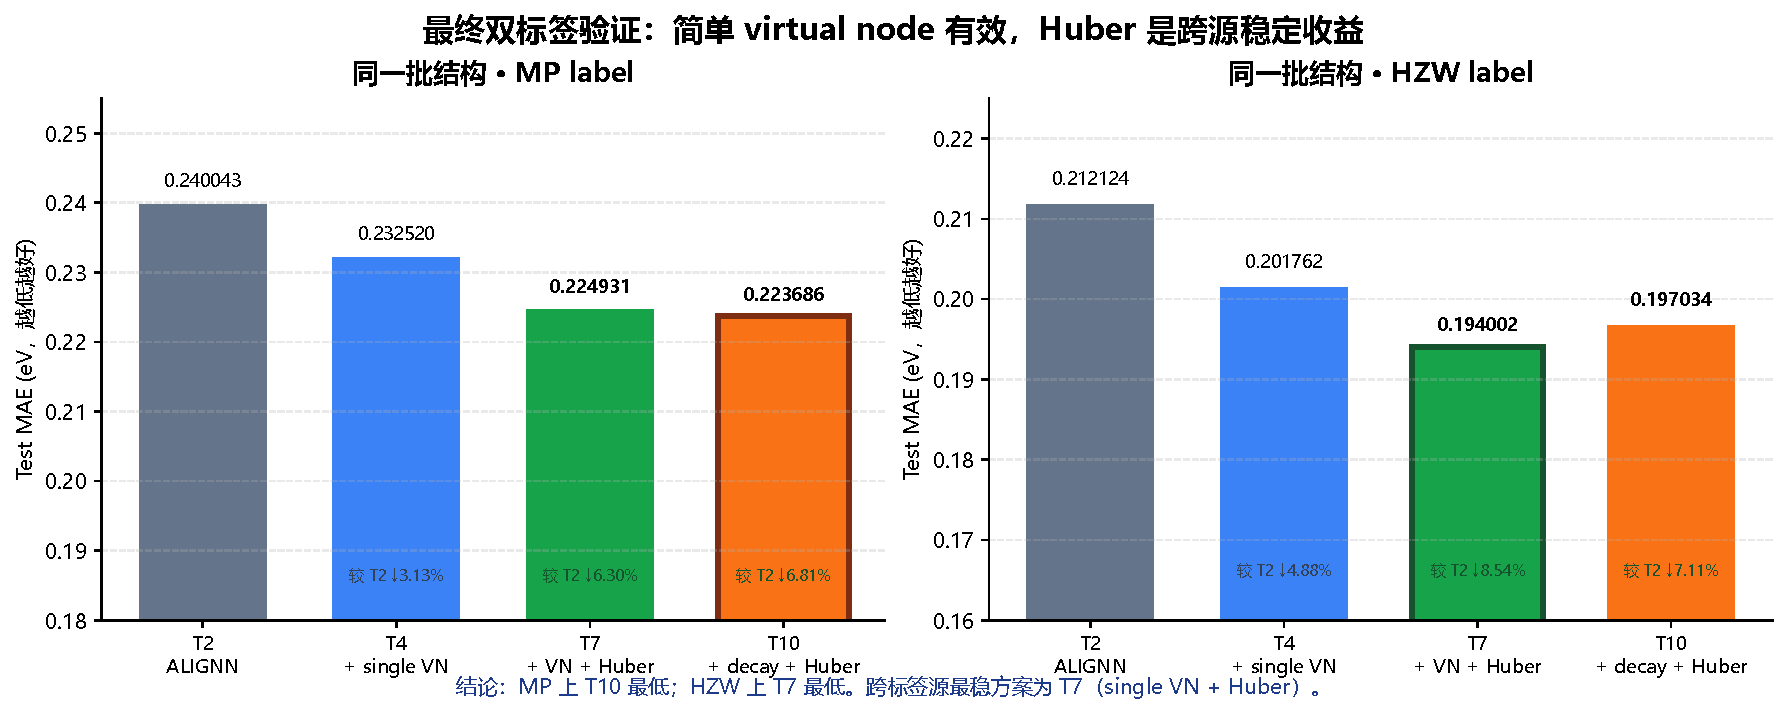
\includegraphics[width=0.96\textwidth]{dual_label_results.pdf}
\speakernote{最终实验使用同一批八万四千五百五十个结构和同一划分，只切换 MP 与 HZW 的 band gap 标签。MP 标签下，ALIGNN 的 MAE 是零点二四零零四三，T10 最低为零点二二三六八六；HZW 标签下，ALIGNN 是零点二一二一二四，T7 最低为零点一九四零零二。T7 相对 ALIGNN 在 MP 上改善百分之六点三，在 HZW 上改善百分之八点五四。因此跨标签源最稳的主张是 single virtual node 加 Huber，而不是某个只在单一标签源最优的复杂机制。}
\end{frame}

% 正文 8
\begin{frame}{当前学术结论与个人研究贡献边界}
\small
\begin{columns}[T,onlytextwidth]
\begin{column}{0.48\textwidth}
\begin{block}{当前可写进论文的三条结论}
\begin{enumerate}
  \item ALIGNN 是最强传统 baseline；single plain VN 是稳定增强。
  \item Huber loss 是跨 MP/HZW 最稳定的进一步收益。
  \item 结构匹配与标签一致性必须分开审计；复杂全局机制具有数据源依赖。
\end{enumerate}
\end{block}
\end{column}
\begin{column}{0.50\textwidth}
\begin{alertblock}{我的主要承担 / 参与}
在导师指导和团队协作下，我主要承担或参与：
\begin{itemize}
  \item 训练框架重建与模型变体实现；
  \item 消融矩阵设计、运行、监控与结果核对；
  \item MP/HZW 数据构建与 structure-first audit；
  \item 图表、结论边界和论文初稿整合。
\end{itemize}
\end{alertblock}
\end{column}
\end{columns}

\begin{center}
不把团队共同成果表述为个人独立成果；署名与权属按实际贡献和团队规则另行确认。
\end{center}
\speakernote{当前论文能站住的结论控制在三条：ALIGNN 是最强传统基线，单 virtual node 稳定有效，Huber 是跨源最稳收益；同时必须把结构匹配和标签一致性分开。个人贡献方面，我在导师指导和团队协作下，主要承担训练框架和变体实现、消融运行与监控、MP HZW 数据审计以及论文图表和初稿整合。我不把团队共同成果说成独立完成，论文署名、代码和数据权属也不在这次汇报中自行决定。}
\end{frame}

% 正文 9
\begin{frame}{成果与验证材料：上半年产物和周期后状态分开统计}
\small
\begin{columns}[T,onlytextwidth]
\begin{column}{0.55\textwidth}
\begin{block}{截至 2026-06-30 的可核验产物}
\begin{itemize}
  \item 25 组完整 `metrics.json` 结果；最终双标签 T 系列各 9 组；
  \item 49 个上半年形成的 YAML 实验配置；
  \item 6 个测试文件；数据导出、审计、队列和监控脚本；
  \item 固定划分的 predictions、history、comparison summary；
  \item 2026-06-11 形成 15 页中文论文初稿 PDF。
\end{itemize}
\end{block}
\end{column}
\begin{column}{0.43\textwidth}
\begin{alertblock}{\postperiod{周期后补充进展}}
\begin{itemize}
  \item 截至 2026-08-25：英文稿 PDF 22 页；
  \item 当前状态：准备投稿，尚未对外宣称已投稿或已接收；
  \item 7—8 月完善不计入上半年完成度，仅用于说明当前状态。
\end{itemize}
\end{alertblock}
\end{column}
\end{columns}
\evidence{结果 CSV/JSON、论文 PDF 元数据、配置和测试文件时间戳；详细路径见附件。}
\speakernote{这一页严格区分周期内和周期后。到六月三十日，仓库中有二十五组完整指标结果，最终双标签 T 系列各九组，四十九个上半年形成的配置、六个测试文件，以及数据导出、审计、队列和监控工具。六月十一日已经生成十五页中文论文初稿。七八月又把英文稿完善到二十二页，目前准备投稿，但这不计入上半年完成度，也不能说成已经投稿或接收。}
\end{frame}

\section{工程与复盘}

% 正文 10
\begin{frame}[shrink=8]{工程任务、交付成果与个人贡献}
\small
\begin{alertblock}{口径边界}
上半年\risk{没有正式工程项目任务书和验收记录}。以下是研究工程化交付能力，不冒充已验收的工程项目绩效。
\end{alertblock}

\begin{tabularx}{\textwidth}{p{2.5cm} p{4.6cm} Y}
\toprule
工程化模块 & 交付内容 & 可复用价值 \\
\midrule
统一训练框架 & CGCNN / ALIGNN / M3GNet runner，指标、预测和 checkpoint 统一输出 & 可比较、可追溯地运行模型矩阵。 \\
配置与消融 & YAML 配置和 E/S/T 编号体系 & 单因素消融与结果复现。 \\
数据流水线 & MP/HZW 导出、匹配、清洗、审计与 metadata & 从原始结构到训练集的口径可追溯。 \\
远程运行保障 & Slurm 队列、watchdog、monitor、失败恢复 & 支撑长时间训练与资源异常定位。 \\
验证资产 & tests、comparison summary、predictions、审计表 & 为论文数字和后续工程验收提供证据。 \\
\bottomrule
\end{tabularx}
\speakernote{按照管理办法，学术进展和工程贡献要分开。这半年没有正式工程项目任务书和验收，所以我不把研究代码说成工程项目绩效。但项目形成了明确的工程化交付能力：统一三类模型的训练输出，用配置管理消融，建立从原始数据到审计训练集的流水线，并用 Slurm 队列、watchdog 和监控保障长任务运行。这些资产可以迁移到下一周期的正式工程任务，但仍需要任务书、负责人和验收标准。}
\end{frame}

% 正文 11
\begin{frame}{未达预期、阴性结果及原因分析}
\scriptsize
\begin{tabularx}{\textwidth}{p{4.1cm} p{4.5cm} Y}
\toprule
未达预期 / 阴性结果 & 主要原因判断 & 如何处理 \\
\midrule
Transformer、attentive VN、dual slot 未稳定超过 simple VN & band gap 更受局部化学主导；复杂机制对数据源和监督噪声更敏感 & 不删除负结果，集中写入消融和局限。 \\
按原子数路由“小结构/大结构专家”不稳 & 原子数不是稳定的“需要额外全局容量”代理；验证阈值不能稳健迁移 & 只作为 diagnostic，不作为正式模型成绩。 \\
Top-$k$ 独立收益不稳定 & 与 Huber 耦合时难以归因；HZW top-$k$-only 反而弱于 simple VN & 将 Huber 作为主贡献，top-$k$ 降为探索。 \\
MP/HZW 上模型排序不一致 & 结构相同但标签类别与数值存在冲突 & 采用 structure-first audit 与同结构双标签验证。 \\
5 月 GPU 任务无法入队 & 账户 QOS 显示 `gres/gpu=0`，属于平台权限问题而非代码问题 & 保存队列与检查脚本，权限恢复后续跑。 \\
周期内未完成投稿 & 结论和数据口径多次变化，论文需要先收敛主张 & 6 月完成中文初稿；7—8 月继续英文完善。 \\
\bottomrule
\end{tabularx}
\speakernote{阴性结果是这次汇报必须主动讲的部分。复杂注意力、双槽位和路由没有稳定超过简单节点；top k 的独立收益也不稳定。原因不是一句“实验失败”，而是 band gap 任务可能更偏局部，复杂机制对标签噪声更敏感，原子数也不是可靠的路由代理。另外五月 GPU 入队失败来自账户 QOS 权限，不是代码错误，但确实造成进度延迟。投稿没有在周期内完成，主要因为模型主张和数据口径需要先收敛，这个偏差由我继续负责补齐。}
\end{frame}

% 正文 12
\begin{frame}[shrink=12]{当前主要问题与风险}
\small
\begin{tabularx}{\textwidth}{p{3.5cm} p{2.0cm} Y}
\toprule
风险 & 影响等级 & 当前应对 \\
\midrule
核心结果仍以固定划分、单次训练为主 & \risk{高} & 为 T4/T7/T10 补多 seed、bootstrap 或 paired error analysis。 \\
relaxed clean 仍保留同类大数值差异 & \risk{高} & 报告双标签口径；用 Huber 与误差分布分析降低过度宣称。 \\
投稿目标和内部审阅尚未最终锁定 & 中 & 先完成导师内审、目标期刊适配和贡献边界确认。 \\
机器学习与量子计算双课题并行 & 中 & 设置主次和固定周时间块，避免两个方向都停留在阅读阶段。 \\
工程进入后任务边界不清 & 中 & 准入后先签任务书，明确负责人、交付物、节点和验收。 \\
计算资源与队列权限波动 & 中 & 申请稳定 GPU 配额；保留失败恢复和可迁移运行方案。 \\
\bottomrule
\end{tabularx}

\begin{alertblock}{最需要避免的情况}
为了赶投稿或同时推进两条方向，扩大结论、跳过复核，或者让工程任务与论文主线互相挤占。
\end{alertblock}
\speakernote{当前最大的学术风险是核心比较仍主要来自固定划分的单次训练，差距较小的结果需要多随机种子或配对误差分析。第二是 relaxed 数据仍有跨源数值差异，所以 Huber 的收益可能部分来自标签噪声，论文必须保持边界。管理上还包括投稿目标没有最终锁定、机器学习和量子计算并行可能分散，以及工程进入后任务不明确。我的应对原则是先锁口径和验收，再增加工作量，而不是同时扩张多个方向。}
\end{frame}

\section{下一周期}

% 正文 13
\begin{frame}[shrink=10]{下一评价周期核心目标与关键里程碑}
\footnotesize
\begin{block}{截至当前的起点（\postperiod{2026-08-30}）}
英文稿已经形成并进入投稿准备；下一周期不是继续无限补实验，而是围绕投稿、可重复验证和新课题形成明确里程碑。
\end{block}

\begin{tabularx}{\textwidth}{p{2.4cm} p{4.8cm} Y}
\toprule
时间 & 核心目标 & 验收标准 \\
\midrule
9 月上旬 & 完成导师内审、目标期刊与格式适配 & 形成修改清单、作者贡献边界和投稿版本。 \\
9 月 & 完成首轮投稿 & 获得投稿编号或明确的投稿记录。 \\
9—10 月 & 补 T4/T7/T10 关键稳健性验证 & 多 seed / bootstrap / paired error 中至少完成一种，并写入补充材料。 \\
10—11 月 & 在胡顺波导师方向确定下一项机器学习课题 & 一页问题定义、数据可得性、baseline 和 8 周实验计划。 \\
9—12 月 & 兼顾刘俊杰导师量子计算课题 & 完成课程/文献基础，并交付一个可运行 benchmark 或阶段报告。 \\
工程准入后 2 周内 & 明确工程任务书 & 写清职责、交付物、负责人、里程碑和验收标准。 \\
12 月 & 形成下一轮可核验材料 & 投稿状态 + 新课题基线 + 量子计算阶段产物 + 工程节点记录。 \\
\bottomrule
\end{tabularx}
\speakernote{下一周期的第一优先级是投稿闭环。以八月二十九日为起点，九月上旬完成导师内审和期刊适配，九月完成首轮投稿；同时只补最关键的稳健性验证，不无限扩展实验。机器学习方面，在胡顺波导师方向确定一个新的、八周可验证的问题。量子计算方面，跟随刘俊杰导师完成课程和文献基础，并交付一个 benchmark 或阶段报告。工程准入后两周内必须形成任务书，避免以模糊参与代替真实交付。}
\end{frame}

% 正文 14
\begin{frame}[shrink=10]{发展路径、工程意向与需要团队协调的支持}
\small
\begin{columns}[T,onlytextwidth]
\begin{column}{0.32\textwidth}
\begin{block}{个人发展路径}
\begin{itemize}
  \item 主线：胡顺波导师方向的机器学习科研；
  \item 协同：刘俊杰导师的量子计算课题；
  \item 路径：\best{学术主线 + 工程准入}，复合型倾向。
\end{itemize}
\end{block}
\end{column}
\begin{column}{0.31\textwidth}
\begin{alertblock}{工程项目意向}
\begin{center}
\Large\best{进入}
\end{center}
前提是明确：项目目标、个人职责、周期里程碑、验收标准与时间占用。
\end{alertblock}
\end{column}
\begin{column}{0.33\textwidth}
\begin{exampleblock}{需要协调的支持}
\begin{itemize}
  \item 稳定 GPU 配额与队列权限；
  \item 论文内部审阅和目标期刊建议；
  \item 双导师课题优先级与时间边界；
  \item 工程准入后的具体任务书和协作人。
\end{itemize}
\end{exampleblock}
\end{column}
\end{columns}

\begin{alertblock}{三句总结}
上半年完成了\best{从模型探索到数据审计和论文初稿的研究闭环}；\\
没有完成的是\risk{周期内投稿和正式工程项目验收}；\\
下一周期以\best{投稿落地、关键复核、新课题基线和工程准入任务书}为验收主线。
\end{alertblock}
\speakernote{发展路径上，我希望继续以胡顺波导师方向的机器学习科研为主，同时兼顾刘俊杰导师的量子计算课题。工程项目意向是进入，但前提是任务、职责、节点和验收清楚。需要团队协调的支持包括稳定 GPU 资源、论文内审和期刊建议、双导师课题的优先级边界，以及工程准入后的具体任务书。总结来说，上半年形成了研究闭环，但投稿和工程验收尚未完成；下一周期要用可核验节点把这两项真正落地。}
\end{frame}

% 附件开始
\reportappendixtrue
\section{证明材料附件}

% 附件 1
\begin{frame}{附件 1：最终 T 系列完整指标}
\tiny
\setlength{\columnsep}{0pt}
\setlength{\tabcolsep}{1.5pt}
\begin{columns}[T,onlytextwidth,totalwidth=\textwidth]
\begin{column}{0.49\textwidth}
\centering
\textbf{MP label（同一批结构）}\\[1mm]
\begin{tabular}{lrrrr}
\toprule
实验 & MAE & RMSE & $R^2$ & Metal F1 \\
\midrule
T1 CGCNN & .366338 & .612696 & .858769 & .788246 \\
T2 ALIGNN & .240043 & .490694 & .909414 & .882637 \\
T3 M3GNet & .285903 & .584315 & .871550 & .889726 \\
T4 single VN & .232520 & .505610 & .903823 & .909240 \\
T6 top-$k$ + Huber & .229585 & .512560 & .901161 & .913312 \\
T7 Huber-only & \textbf{.224931} & .503546 & .904607 & .911331 \\
T8 top-$k$-only & .230402 & .496074 & .907417 & .905809 \\
T9 warmup + Huber & .226028 & .495817 & .907513 & .914071 \\
T10 decay + Huber & \textbf{.223686} & .497333 & .906946 & \textbf{.915455} \\
\bottomrule
\end{tabular}
\end{column}
\begin{column}{0.49\textwidth}
\centering
\textbf{HZW label（同一批结构）}\\[1mm]
\begin{tabular}{lrrrr}
\toprule
实验 & MAE & RMSE & $R^2$ & Metal F1 \\
\midrule
T1 CGCNN & .338152 & .565454 & .878497 & .788237 \\
T2 ALIGNN & .212124 & .436147 & .927713 & .890299 \\
T3 M3GNet & .256572 & .535916 & .890859 & .892629 \\
T4 single VN & .201762 & .448621 & .923519 & .909613 \\
T6 top-$k$ + Huber & .198584 & .447143 & .924022 & .913786 \\
T7 Huber-only & \textbf{.194002} & .445837 & .924465 & .915401 \\
T8 top-$k$-only & .202603 & .448503 & .923559 & .909881 \\
T9 warmup + Huber & .197707 & .448776 & .923466 & \textbf{.916846} \\
T10 decay + Huber & .197034 & .453592 & .921815 & .913209 \\
\bottomrule
\end{tabular}
\end{column}
\end{columns}
\vspace{2mm}
\begin{block}{引用规则}
T7 是跨源最稳方案；T10 只应表述为 MP label 特化最优。T6/T9 同时包含 Huber，不能把收益单独归因于 top-$k$。
\end{block}
\speakernote{附件一是完整 T 系列指标，正常十五分钟不主动讲。如果老师追问某个模型的 RMSE、R 方或 Metal F1，可以在这里核对。需要强调的引用规则是：T7 是跨标签源最稳的方案；T10 只在 MP 标签上取得最低 MAE；包含 Huber 的 T6 和 T9 不能用来单独证明 top k 有效。}
\end{frame}

% 附件 2
\begin{frame}{附件 2：数据审计口径与证据路径}
\scriptsize
\begin{tabularx}{\textwidth}{p{3.6cm} p{2.2cm} Y}
\toprule
审计项 & 数量 & 证据文件 \\
\midrule
可审计总记录 & 95,462 & `mp\_hzw\_structure\_first\_summary.json` \\
结构匹配 & 92,787 & `mp\_hzw\_structure\_matched\_all.csv` \\
缺 MP 记录 & 2,636 & `mp\_hzw\_missing\_mp\_record.csv` \\
结构不匹配 & 39 & `mp\_hzw\_structure\_unmatched\_all.csv` \\
MP metal / HZW nonmetal & 3,142 & `mp\_hzw\_matched\_mp\_metal\_hzw\_nonmetal.csv` \\
MP nonmetal / HZW metal & 3,046 & `mp\_hzw\_matched\_mp\_nonmetal\_hzw\_metal.csv` \\
同类 gap 差 $>1$ eV & 1,121 & `mp\_hzw\_matched\_same\_class\_gap\_diff\_gt\_1ev.csv` \\
最终 relaxed equal-atoms & 84,550 & 双标签数据 metadata 与固定 split \\
\bottomrule
\end{tabularx}

\begin{alertblock}{保密与归档}
PPT 只展示统计摘要；原始大表、源码、服务器信息和未公开论文全文采用受控查验，不随普通 PPT 对外传播。
\end{alertblock}
\speakernote{附件二给出数据审计的证据入口。所有数字都能回到 JSON 汇总或 CSV 明细。按照管理办法，PPT 只展示统计摘要，不把原始大表、服务器信息、敏感源码和未公开论文全文放进普通归档。如果需要复核，我可以在受控环境中按文件逐项展示。}
\end{frame}

% 附件 3
\begin{frame}{附件 3：代码、实验、论文与报告索引}
\scriptsize
\begin{tabularx}{\textwidth}{p{2.5cm} p{5.0cm} Y}
\toprule
类别 & 代表文件 / 目录 & 可验证内容 \\
\midrule
模型实现 & \path{faithful_gnn/alignn_variants.py}、各 runner & virtual node、physics、routing、Huber/top-$k$/decay 等实现。 \\
实验配置 & \path{configs/}、\path{configs/mp/} & E/S/T 系列的参数、数据口径和模型定义。 \\
数据流水线 & \path{export_mp_hzw_*}、\path{audit_mp_hzw_*} & 导出、结构匹配、清洗、审计和 metadata。 \\
运行保障 & \path{scripts/slurm_*}、watchdog、monitor & 远程队列、日志、失败恢复和资源检查。 \\
结果证据 & \path{results/.../metrics.json}、predictions、comparison summary & MAE、RMSE、$R^2$、Metal F1、训练曲线和逐样本误差。 \\
测试 & \path{tests/} & size gate、router、dataset export、top-$k$/Huber 等行为检查。 \\
论文 & \path{gnn_bandgap_research_paper_draft.pdf} & 2026-06-11 的 15 页中文初稿。 \\
周期后论文 & \path{gnn_bandgap_research_paper_draft_en.pdf} & 2026-08-25 的 22 页英文稿；准备投稿。 \\
阶段报告 & weekly/progress/final/history report & 研究过程、结果口径和阶段汇报记录。 \\
\bottomrule
\end{tabularx}
\speakernote{附件三是产物索引，用于回答材料是否可验证。模型实现、配置、数据流水线、运行保障、结果、测试和论文都有对应文件。这里列的是证据入口，不代表所有产物都由我独立完成；具体贡献仍按代码记录、实验分工和团队确认来界定。}
\end{frame}

\end{document}
